
%!TEX root = handout.tex

\newpage
\section{Label-free quantification of peptides}
\label{sec:lfq}

\subsection{Introduction}

In this chapter, we will build a workflow with OpenMS / KNIME to quantify a label-free experiment. 
Label-free quantification is a method aiming to compare the relative amounts of proteins or peptides in two or more samples.
We will start from the minimal workflow of the last chapter and, step-by-step, build a label-free quantification workflow.

\subsection{Peptide Identification}
\label{Peptide_Identification}

As a start, we will extend the minimal workflow so that it performs a peptide identification using the OMSSA~\cite{Geer:2004p285} search engine. Since OpenMS version 1.10, OMSSA is included in the OpenMS installation, so you do not need to download and install it yourself.

\begin{itemize}
\item Let's start by replacing the input files in our \KNIMENODE{Input Files} node by the three mzML files in \directory{Example\_Data / Labelfree / datasets / lfq\_spikein\_dilution\_1-3.mzML}. This is a reduced toy dataset where each of the three runs contains a constant background of \textit{S. pyogenes} peptides as well as human spike-in peptides in different concentrations.~\cite{Chawade:2015}
\item Instead of FileInfo, we want to perform OMSSA identification, so we simply replace the \KNIMENODE{FileInfo} node with the \KNIMENODE{OMSSAAdapter} node \menu{Community Nodes > OpenMS > Identification}, and we are almost done. Just make sure you have connected the \KNIMENODE{ZipLoopStart} node with the \texttt{in} port of the \KNIMENODE{OMSSAAdapter} node.
\item OMSSA, like most mass spectrometry identification engines, relies on searching the input spectra against sequence databases. Thus, we need to introduce a search database input. As we want to use the same search database for all of our input files, we can just add a single \KNIMENODE{Input File} node to the workflow and connect it directly with the \KNIMENODE{OMSSAAdapter} \texttt{database} port. KNIME will automatically reuse this Input node each time a new ZipLoop iteration is started. In order to specify the database, select \directory{Example\_Data / Labelfree / databases / \\ s\_pyo\_sf370\_potato\_human\_target\_decoy\_with\_contaminants.fasta}, and we have a very basic peptide identification workflow.
%\note{We recommend to choose a different output directory every time you extend and run your pipeline again.}
\note{You might also want to save your new identification workflow under a different name. Have a look at \cref{sec:duplicate-wf} for information on how to create copies of workflows.}
\item The result of a single OMSSA run is basically a number of peptide-spectrum-matches (PSM) with a score each, and these will be stored in an idXML file. Now we can run the pipeline and after execution is finished, we can have a first look at the results: just open the input files folder with a file browser and from there open an mzML file in \OPENMSTOOL{TOPPView}.
\item Here, you can annotate this spectrum data file with the peptide identification results. Choose \menu{Tools > Annotate with identification} from the menu and select the idXML file that \KNIMENODE{OMSSAAdapter} generated (it is located within the output directory that you specified when starting the pipeline).
\item On the right, select the tab \menu{Identification view}. Using this view, you can see all identified peptides and browse the corresponding MS2 spectra.
\note{Opening the output file of \KNIMENODE{OMSSAAdapter} (the idXML file) directly is also possible, but the direct visualization of an idXML file is less useful.}
\item The search results stored in the idXML file can also be read back into a KNIME table for inspection and subsequent analyses: Add a \KNIMENODE{TextExporter} node from \menu{Community Nodes > OpenMS > File Handling} to your workflow and connect the output port of your \KNIMENODE{OMSSAAdapter} (the same port your \KNIMENODE{ZipLoopEnd} is connected to) to its input port. This tool will convert the idXML file to a more human-readable text file which can also be read into a KNIME table using the \KNIMENODE{IDTextReader} node. Add an \KNIMENODE{IDTextReader} node (\menu{Community Nodes > OpenMS > Conversion}) after \KNIMENODE{TextExporter} and execute it. Now you can right-click \KNIMENODE{IDTextReader} and select \menu{ID Table} to browse your peptide identifications.
\item From here, you can use all the tools KNIME offers for analyzing the data in this table. As a simple example, you could add a \KNIMENODE{Histogram} node (from category \menu{Data Views}) node after \KNIMENODE{IDTextReader}, double-click it, select \textit{peptide\_charge} as binning column, hit \menu{OK}, and execute it. Right-clicking and selecting \menu{View: Histogram view} will open a plot showing the charge state distribution of your identifications.
\end{itemize}

In the next step, we will tweak the parameters of OMSSA to better reflect the instrument's accuracy. Also, we will extend our pipeline with a false discovery rate (FDR) filter to retain only those identifications that will yield an FDR of $<$ 1 \%.

\begin{itemize}
\item
Open the configuration dialog of \KNIMENODE{OMSSAAdapter}.
The dataset was recorded using an LTQ Orbitrap XL mass spectrometer, so we can set the precursor mass tolerance to a smaller value, say 10 ppm.
Set \textit{precursor\textunderscore mass\textunderscore tolerance} to 10 and \\ \textit{precursor\textunderscore error\textunderscore units} to \textit{ppm}.
\note{Whenever you change the configuration of a node, the node as well as all its successors will be reset to the Configured state (all node results are discarded and need to be recalculated by executing the nodes again).}
\item
Set \textit{max\_precursor\_charge} to 5, in order to also search for peptides with charges up to 5.
\item
Add \textit{Carbamidomethyl (C)} as fixed modification and \textit{Oxidation (M)} as variable modification.
\note{To add a modification click on the empty value field in the configuration dialog to open the list editor dialog.
In the new dialog click \menu{Add}.
Then select the newly added modification to open the drop down list where you can select the correct modification.}
\item
A common step in analyis is to search not only against a regular protein database, but to also search against a decoy database for FDR estimation.
The fasta file we used before already contains such a decoy database.
For OpenMS to know which OMSSA PSM came from which part of the file (i.e. target versus decoy), we have to index the results.
Therefore, extend the workflow with a \KNIMENODE{PeptideIndexer} node \menu{Community Nodes > OpenMS > ID Processing}.
This node needs the idXML as input as well as the database file.
\note{You can direct the files of an \KNIMENODE{Input File} node to more than just one destination port.}
\item
The decoys in the database are prefixed with ``DECOY\_'', so we have to set \textit{decoy\_string} to \textit{DECOY\_} and \textit{decoy\_string\_position} to \textit{prefix} in the configuration dialog of \KNIMENODE{PeptideIndexer}.
\item
Now we can go for the FDR estimation, which the \KNIMENODE{FalseDiscoveryRate} node will calculate for us (you will find it in \menu{Community Nodes > OpenMS > ID Processing}).
As we have a combined search database and thus only one idXML per mzML we will only use the \textit{in} port of the \KNIMENODE{FalseDiscoveryRate} node.
\item
In order to set the FDR level to $1\%$, we need an \KNIMENODE{IDFilter} node from \menu{Community Nodes > OpenMS > ID Processing}.
Configuring its parameter \textit{score $\rightarrow$ pep} to $0.01$ will do the trick.
The FDR calculations (embedded in the idXML) from the \KNIMENODE{FalseDiscoveryRate} node will go into the \textit{in} port of the \KNIMENODE{IDFilter} node.
\item
Execute your workflow and inspect the results using \KNIMENODE{IDTextReader} like you did before.
How many peptides did you identify at this FDR threshold?
\note{The finished identification workflow is now sufficiently complex that we might want to encapsulate it in a Meta node.
For this, select all nodes inside the ZipLoop (including the \KNIMENODE{Input File} node) and right-click to select \menu{Collapse into Meta node} and name it ID.
Meta nodes are useful when you construct even larger workflows and want to keep an overview.}
\end{itemize}

\begin{figure}[htbp]
  \centering
  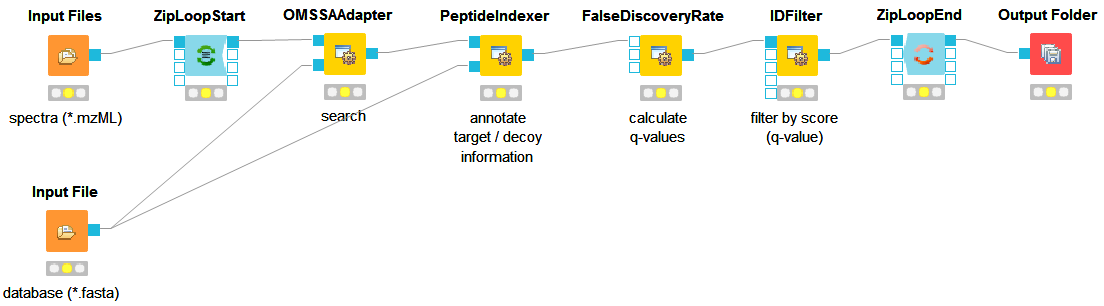
\includegraphics[width=\textwidth]{graphics/labelfree/PepIdFDR.png}
  \caption{OMSSA ID pipeline including FDR filtering.}
  \label{fig:id_fdr}
\end{figure}

\subsubsection{Bonus task: identification using several search engines}
\note{If you are ahead of the tutorial or later on, you can further improve your FDR identification workflow by a so-called consensus identification using several search engines. Otherwise, just continue with section \ref{Labelfree_Quantification}.}
It has become widely accepted that the parallel usage of different search engines can increase peptide identification rates in shotgun proteomics experiments. The ConsensusID algorithm is based on the calculation of posterior error probabilities (PEP) and a combination of the normalized scores by considering missing peptide sequences.

\begin{itemize}
\item
Next to the \KNIMENODE{OMSSAAdapter} add a \KNIMENODE{XTandemAdapter} \\
\menu{Community Nodes > OpenMS > Identification} node and set its parameters and ports analogously to the \KNIMENODE{OMSSAAdapter}. In XTandem, to get more evenly distributed scores, we decrease the number of candidates a bit by setting the precursor mass tolerance to 5 ppm and the fragment mass tolerance to 0.1 Da.
\item
To calculate the PEP, introduce each a \KNIMENODE{IDPosteriorErrorProbability} \menu{Community Nodes > OpenMS > ID Processing} node to the output of each ID engine adapter node.
This will calculate the PEP to each hit and output an updated idXML.
\item
To create a consensus, we must first merge these two files with a \KNIMENODE{FileMerger} node \menu{Community Nodes > GenericKnimeNodes > Flow} so we can then merge the corresponding IDs with a \KNIMENODE{IDMerger} \menu{Community Nodes > OpenMS > File Handling}.
\item
Now we can create a consensus identification with the \KNIMENODE{ConsensusID} \menu{Community Nodes > OpenMS > ID Processing} node.
We can connect this to the \KNIMENODE{PeptideIndexer} and go along with our existing FDR filtering.
\note{By default, X!Tandem takes additional enzyme cutting rules into consideration (besides the specified tryptic digest). Thus for the tutorial files, you have to set PeptideIndexer's \textit{enzyme $\rightarrow$ specificity} parameter to \texttt{none} to accept X!Tandems non-tryptic identifications as well.}
\end{itemize}

\begin{figure}[htbp]
  \centering
  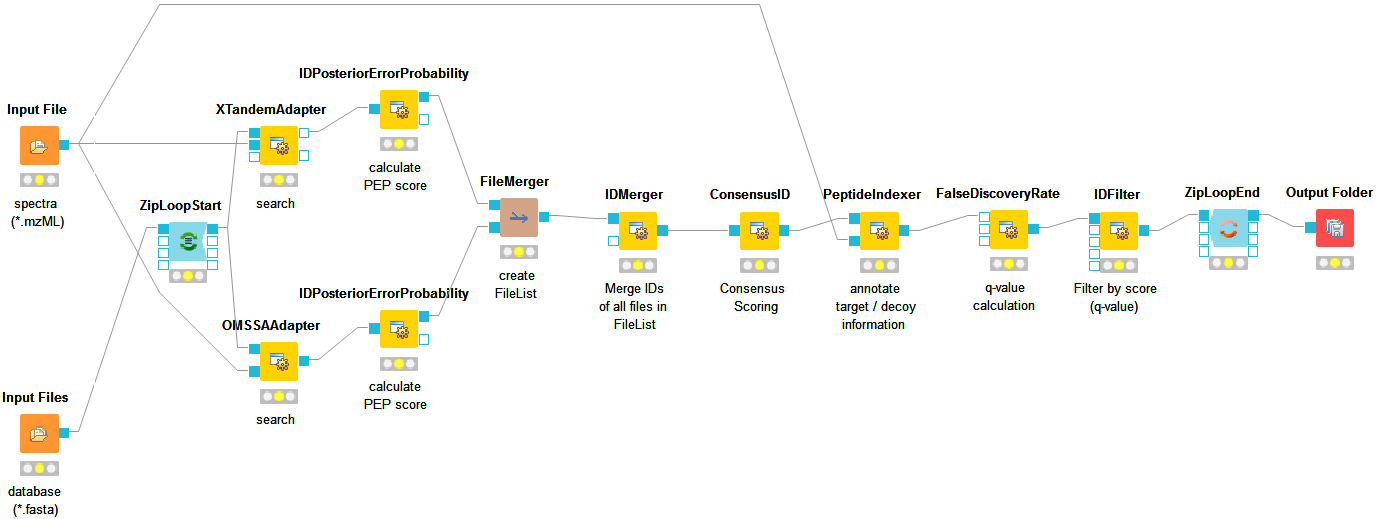
\includegraphics[width=\textwidth]{graphics/labelfree/PepConsensusId.png}
  \caption{Complete consensus identification workflow.}
  \label{fig:consensusid}
\end{figure}

\newpage
\subsection{Quantification}
\label{Labelfree_Quantification}

Now that we have successfully constructed a peptide identification pipeline, we can add quantification capabilities to our workflow.

\begin{itemize}
\item
Add a \KNIMENODE{FeatureFinderCentroided} node from \menu{Community Nodes > OpenMS > Quantitation} which gets input from the first output port of the \KNIMENODE{ZipLoopStart} node. Also, add an \KNIMENODE{IDMapper} node (from \menu{Community Nodes > OpenMS > ID Processing}) which receives input from the \KNIMENODE{FeatureFinderCentroided} node and the ID Meta node (or \KNIMENODE{IDFilter} node if you haven't used the Meta node).
The output of the \KNIMENODE{IDMapper} is then connected to an \textit{in} port of the \KNIMENODE{ZipLoopEnd} node.
\item
\KNIMENODE{FeatureFinderCentroided} finds and quantifies peptide ion signals contained in the MS1 data.
It reduces the entire signal, i.e., all peaks explained by one and the same peptide ion signal, to a single peak at the maximum of the chromatographic elution profile of the monoisotopic mass trace of this peptide ion and assigns an overall intensity.
\item
\KNIMENODE{FeatureFinderCentroided} produces a featureXML file as output, containing only quantitative information of so-far unidentified peptide signals.
In order to annotate these with the corresponding ID information, we need the \KNIMENODE{IDMapper} node.
\item Run your pipeline and inspect the results of the \KNIMENODE{IDMapper} node in TOPPView. Open the mzML file of your data to display the raw peak intensities.
\item To assess how well the feature finding worked, you can project the features contained in the featureXML file on the raw data contained in the mzML file. To this end, open the featureXML file in TOPPView by clicking on \menu{File > Open file} and add it to a new layer (\menu{Open in > New layer}). The features are now visualized on top of your raw data. If you zoom in on a small region, you should be able to see the individual boxes around features that have been detected (see Fig.~\ref{fig:ff_featurexml}). If you hover over the the feature centroid (small circle indicating the chromatographic apex of monoisotopic trace) additional information of the feature is displayed.

\begin{figure}[!htbp]
  \centering
  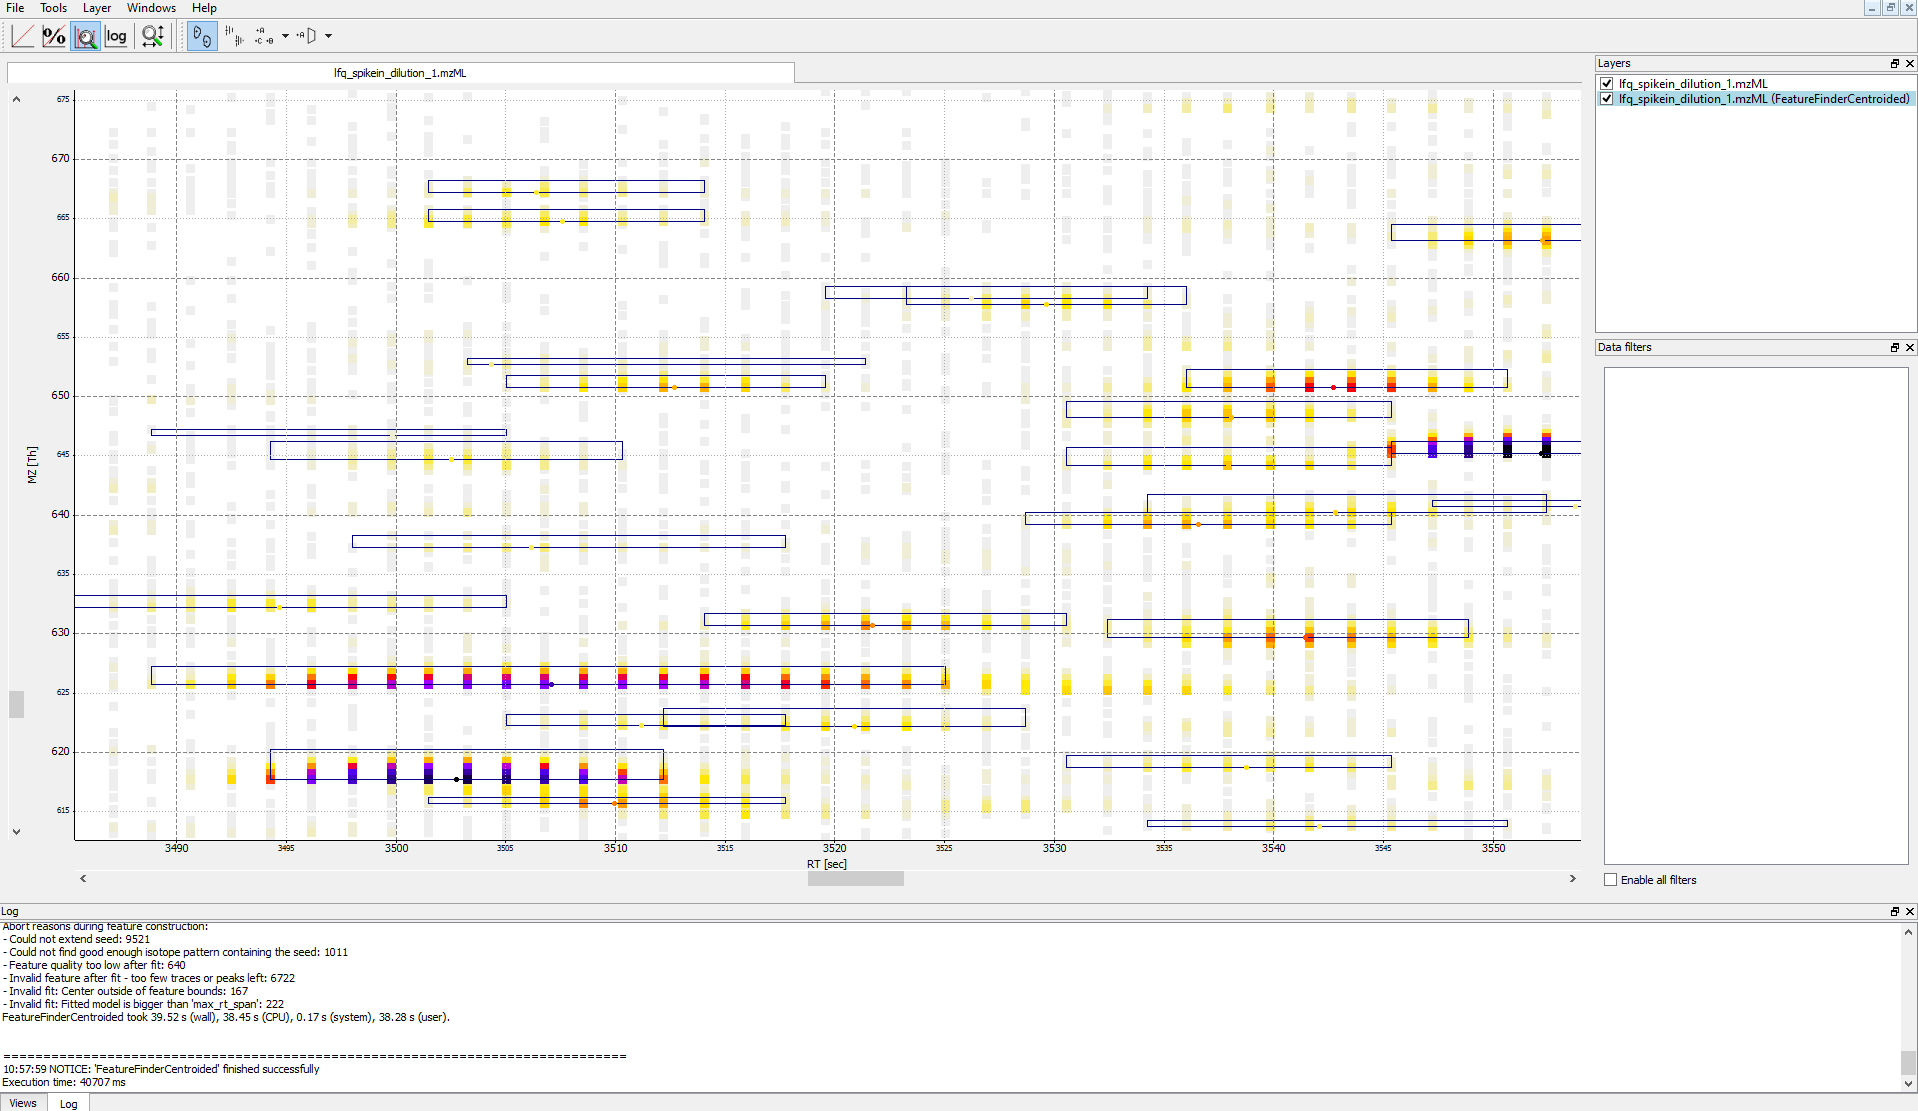
\includegraphics[width=0.85\textwidth]{graphics/labelfree/featureXML.png}
  \caption{Visualization of detected features (boxes) in TOPPView.}
  \label{fig:ff_featurexml}
\end{figure}

\note{The chromatographic RT range of a feature is about 30-60~s and its m/z range around 2.5 m/z in this dataset. If you have trouble zooming in on a feature, select the full RT range and zoom only into the m/z dimension by holding down \keys{\ctrlwin} (\keys{cmd \cmd} on macOS) and repeatedly dragging a narrow box from the very left to the very right.}
\item
You can see which features were annotated with a peptide identification by first selecting the featureXML file in the \texttt{Layers} window on the upper right side and then clicking on the icon with the letters A, B and C on the upper icon bar.
Now, click on the small triangle next to that icon and select \texttt{Peptide identification}.
\end{itemize}

\begin{figure}[htbp]
  \centering
  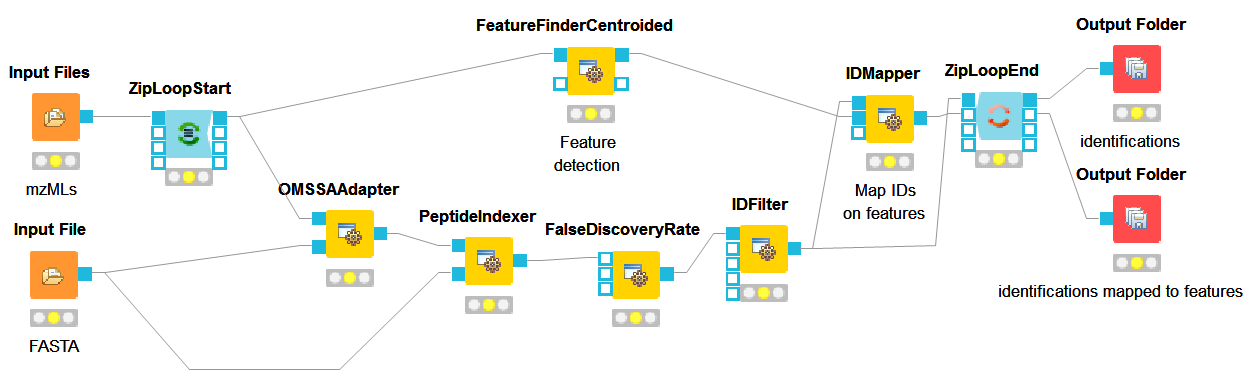
\includegraphics[width=\textwidth]{graphics/labelfree/PepQuantIdNoAlign.png}
  \caption{Extended workflow featuring peptide identification and quantification.}
  \label{fig:ff_idmapping}
\end{figure}

\subsection{Combining quantitative information across several label-free experiments}
\label{Combining}

So far, we successfully performed peptide identification as well as quantification on individual LC-MS runs. For differential label-free analyses, however, we need to identify and quantify corresponding signals in different experiments and link them together to compare their intensities. Thus, we will now run our pipeline on all three available input files and extend it a bit further, so that it is able to find and link features across several runs.

\begin{figure}[htbp]
  \centering
  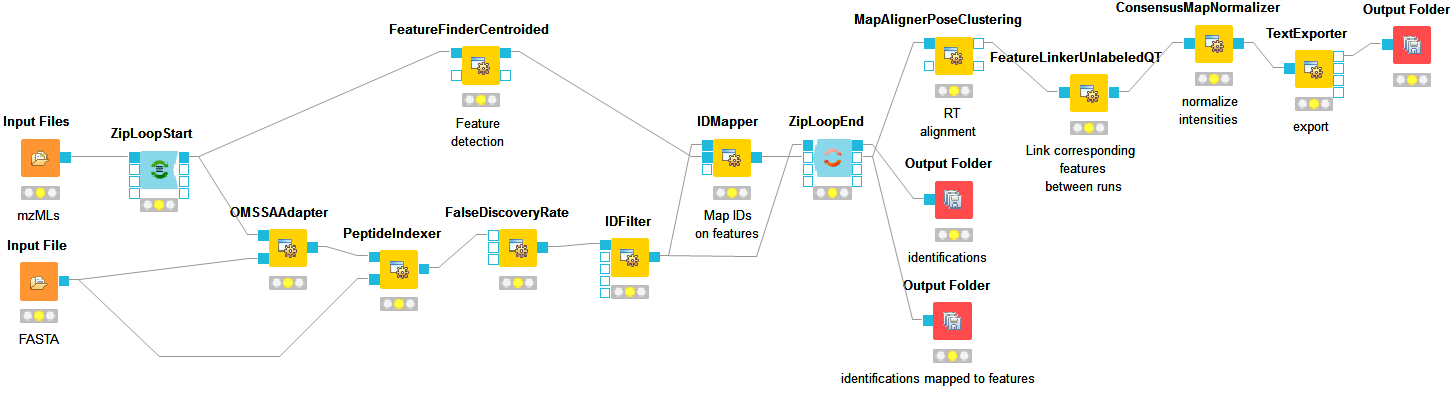
\includegraphics[width=\textwidth]{graphics/labelfree/PepQuantId.png}
  \caption{Complete identification and label-free quantification workflow.}
  \label{fig:complete_without_consensusid}
\end{figure}

\begin{itemize}
    \item To find features across several maps, we first have to align them to correct for retention time shifts between the different label-free measurements. With the \KNIMENODE{MapAlignerPoseClustering} in \menu{Community Nodes > OpenMS > Map Alignment}, we can align corresponding peptide signals to each other as closely as possible by applying a transformation in the RT dimension. \note{\KNIMENODE{MapAlignerPoseClustering} consumes several featureXML files and its output should still be several featureXML files containing the same features, but with the transformed RT values. In its configuration dialog, make sure that \textit{OutputTypes} is set to featureXML.}
    \item With the \KNIMENODE{FeatureLinkerUnlabeledQT} node in \menu{Community Nodes > OpenMS > Map Alignment}, we can then perform the actual linking of corresponding features. Its output is a consensusXML file containing linked groups of corresponding features across the different experiments.
    \item Since the overall intensities can vary a lot between different measurements (for example, because the amount of injected analytes was different), we apply the \KNIMENODE{ConsensusMapNormalizer} in \menu{Community Nodes > OpenMS > Map Alignment} as a last processing step. Configure its parameters with setting \textit{algorithm\_type} to \texttt{median}. It will then normalize the maps in such a way that the median intensity of all input maps is equal.
    \item Finally, we export the resulting normalized consensusXML file to a csv format using \KNIMENODE{TextExporter}. Connect its out port to a new \KNIMENODE{Output Folder} node.
    \note{You can specify the desired column separation character in the parameter settings (by default, it is set to `` '' (a space)). The output file of \KNIMENODE{TextExporter} can also be opened with external tools, e.g., Microsoft Excel, for downstream statistical analyses.}
\end{itemize}

\subsubsection{Basic data analysis in KNIME}

For downstream analysis of the quantification results within the KNIME environment, you can use the \KNIMENODE{ConsensusTextReader} node in \menu{Community Nodes > OpenMS > Conversion} instead of the \KNIMENODE{Output Folder} node to convert the output into a KNIME table (indicated by a triangle as output port). 
After running the node you can view the KNIME table by right-clicking on the \KNIMENODE{ConsensusTextReader} and selecting \menu{Consensus Table}.
Every row in this table corresponds to a so-called consensus feature, i.e., a peptide signal quantified across several runs. The first couple of columns describe the consensus feature as a whole (average RT and m/z across the maps, charge, etc.). The remaining columns describe the exact positions and intensities of the quantified features separately for all input samples (e.g., intensity\_0 is the intensity of the feature in the first input file). The last 11 columns contain information on peptide identification.

\begin{figure}[htbp]
  \centering
  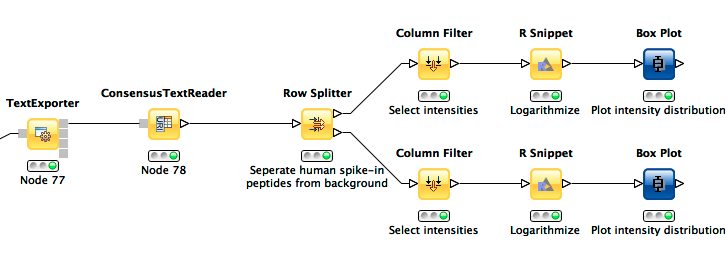
\includegraphics[width=0.85\textwidth]{graphics/labelfree/data_analysis.png}
  \caption{Simple KNIME data analysis example for LFQ.}
  \label{fig:lfq_data_analysis}
\end{figure}

\begin{itemize}
    \item Now, let's say we want to plot the log intensity distributions of the human spike-in peptides for all input files. In addition, we will plot the intensity distributions of the background peptides.
    \item As shown in Fig. \ref{fig:lfq_data_analysis}, add a \KNIMENODE{Row Splitter} node (\menu{Data Manipulation > Row > Filter}) after \KNIMENODE{ConsensusTextReader}. Double-click it to configure. The human spike-in peptides have accessions starting with ``hum''. Thus, set the column to apply the test to: \textit{accessions}, select pattern matching as matching criterion, enter \textit{hum*} into the corresponding text field, and check the \textit{contains wild cards} box. Press OK and execute the node.
    \item \KNIMENODE{Row Splitter} produces two output tables: the first one contains all rows from the input table matching the filter criterion, and the second table contains all other rows. You can inspect the tables by right-clicking and selecting \textit{Filtered} and \textit{Filtered Out}. The former table should now only contain peptides with a human accession, whereas the latter should contain all remaining peptides (including unidentified ones).
    \item Now, since we only want to plot intensities, we can add a \KNIMENODE{Column Filter} node \\ \menu{Data Manipulation > Column > Filter}, connect its input port to the \textit{Filtered} output port of the \KNIMENODE{Row Filter}, and open its configuration dialog. We could either manually select the columns we want to keep, or, more elegantly, select \textit{Wildcard/Regex Selection} and enter \textit{intensity\_?} as the pattern. KNIME will interactively show you which columns your pattern applies to while you're typing.
    \item Since we want to plot log intensities, we will now compute the log of all intensity values in our table. The easiest way to do this in KNIME is a small piece of R code. Add an \KNIMENODE{R Snippet} node \menu{R} after \KNIMENODE{Column Filter} and double-click to configure. In the \textit{R Script} text editor, enter the following code:
        \begin{lstlisting}
            x <- knime.in       # store copy of input table in x
            x[x == 0] <- NA     # replace all zeros by NA (= missing value)
            x <- log10(x)       # compute log of all values
            knime.out <- x      # write result to output table
        \end{lstlisting}
    \item Now we are ready to plot! Add a \KNIMENODE{Box Plot} node \menu{Views} after the \KNIMENODE{R Snippet} node, execute it, and open its view. If everything went well, you should see a significant fold change of your human peptide intensities across the three runs.
    \item In order to verify that the concentration of background peptides is constant in all three runs, you can just copy and paste the three nodes after \KNIMENODE{Row Splitter} and connect the duplicated \KNIMENODE{Column Filter} to the second output port (\textit{Filtered Out}) of \KNIMENODE{Row Splitter}, as shown in Fig. \ref{fig:lfq_data_analysis}. Execute and open the view of your second \KNIMENODE{Box Plot}.
    \item That's it! You have constructed an entire identification and label-free quantification workflow including a simple data analysis using KNIME!
\end{itemize}
 
%The output of the node should now be compatible with most of the nodes of the KNIME base as well as the R nodes, which leaves room for you to play with these.
%Possible analyses include:

%\begin{task}
%Filtering (\KNIMENODE{Row Filter}, \KNIMENODE{Rule-based Row Filter}) or grouping (\KNIMENODE{GroupBy}; e.g. by charge) of the identified peptides/proteins.
%\end{task}
%\begin{task}
%Statistical analysis with \KNIMENODE{R Snippet} nodes or the nodes from the KNIME Statistics package.
%\end{task}
%\begin{task}
%Plotting of the (cumulative) distribution of q-values, quality scores (of the consensus features) or other peptide hit properties using \KNIMENODE{R View} nodes or the standard KNIME nodes for plotting (which include interactive functionality).
%\end{task}

\subsection{Identification \& Quantification of the iPRG2015 data with subsequent MSstats analysis}
Advanced downstream data analysis of quantitative mass spectrometry-based proteomics data can be performed using MSstats ~\cite{Choi2014MSstats}. This tool can be combined with an OpenMS preprocessing pipeline (e.g. in KNIME). The OpenMS experimental design is used to present the data in an MSstats-conformant way for the analysis. In this tutorial, we would like to present an example how to utilize these resources when working with quantitative label-free data. Therefore, we describe how to use OpenMS and MSstats in the analysis of the ABRF iPRG2015 dataset~\cite{Choi2017iPRG}.

\note{Due to runtime constrictions in the tutorial session only the conversion process and the downstream analysis will be presented in further detail.}

\subsubsection{Excursion MSstats}
The R package MSstats can be used for statistical relative quantification of proteins and peptides in mass spectrometry-based proteomics. Supported are label-free as well as labeled experiments in combination with data-dependent, targeted and data-independent acquisition. Inputs can be identified and quantified entities (peptides or proteins) and the output is a list of differentially abundant entities, or summaries of their relative abundance. It depends on accurate feature detection, identification and quantification which can be performed e.g. by an OpenMS workflow. 

\noindent In general MSstats can be used for data processing \& visualization, as well as statistical modeling \& inference. Please see ~\cite{Choi2014MSstats} and \url{http://msstats.org} for further information.

\subsubsection{Dataset}
The iPRG (Proteome Informatics Research Group) dataset from the study in 2015, as described in ~\cite{Choi2017iPRG}, aims at evaluating the effect of statistical analysis software on the accuracy of results on a label-free quantification experiment on proteins. The data is based on four artificial samples of known composition (background: 200\,ng \emph{S. cerevisiae}), which were spiked with different quantities of individual digested proteins, whose identifiers were masked for the competition as yeast proteins in the provided database (see table \ref{t:dataset_iPRG}).

\renewcommand{\arraystretch}{1.2} %% increase row height a little
\begin{table}[!ht]
\centering
\small
\caption{Samples (background: 200\,ng \emph{S. cerevisiae}) with spiked-in proteins in different quantities [fmols]}
\label{t:dataset_iPRG}
\begin{tabular}{llll|llll}
  &                          &                              &                                      & \multicolumn{4}{c}{Samples}            \\
\hline 
  & \multicolumn{1}{c}{Name} & \multicolumn{1}{c}{Origin}   & \multicolumn{1}{c}{Molecular Weight} & \multicolumn{1}{c}{1} & 2   & 3  & 4   \\
\hline
\hline
A & Ovalbumin                & \textit{Egg White}   & 45 KD                                 & 65                    & 55  & 15 & 2   \\
\hline
B & Myoglobin                & \textit{Equine Heart}        & 17 KD                                 & 55                    & 15  & 2  & 65  \\
\hline
C & Phosphorylase b          & \textit{Rabbit Muscle}       & 97 KD                                 & 15                    & 2   & 65 & 55  \\
\hline
D & Beta-Glactosidase        & \textit{Escherichia Coli}    & 116 KD                                & 2                     & 65  & 55 & 15  \\
\hline
\hline
E & Bovine Serum Albumin     & \textit{Bovine Serum}        & 66 KD                                 & 11                    & 0.6 & 10 & 500 \\
\hline
F & Carbonic Anhydrase       & \textit{Bovine Erythrocytes} & 29 KD                                 & 10                    & 500 & 11 & 0.6 \\
\hline
\end{tabular}
\end{table}

\subsubsection{Identification and Quantification}

\begin{figure}[htbp]
  \centering
  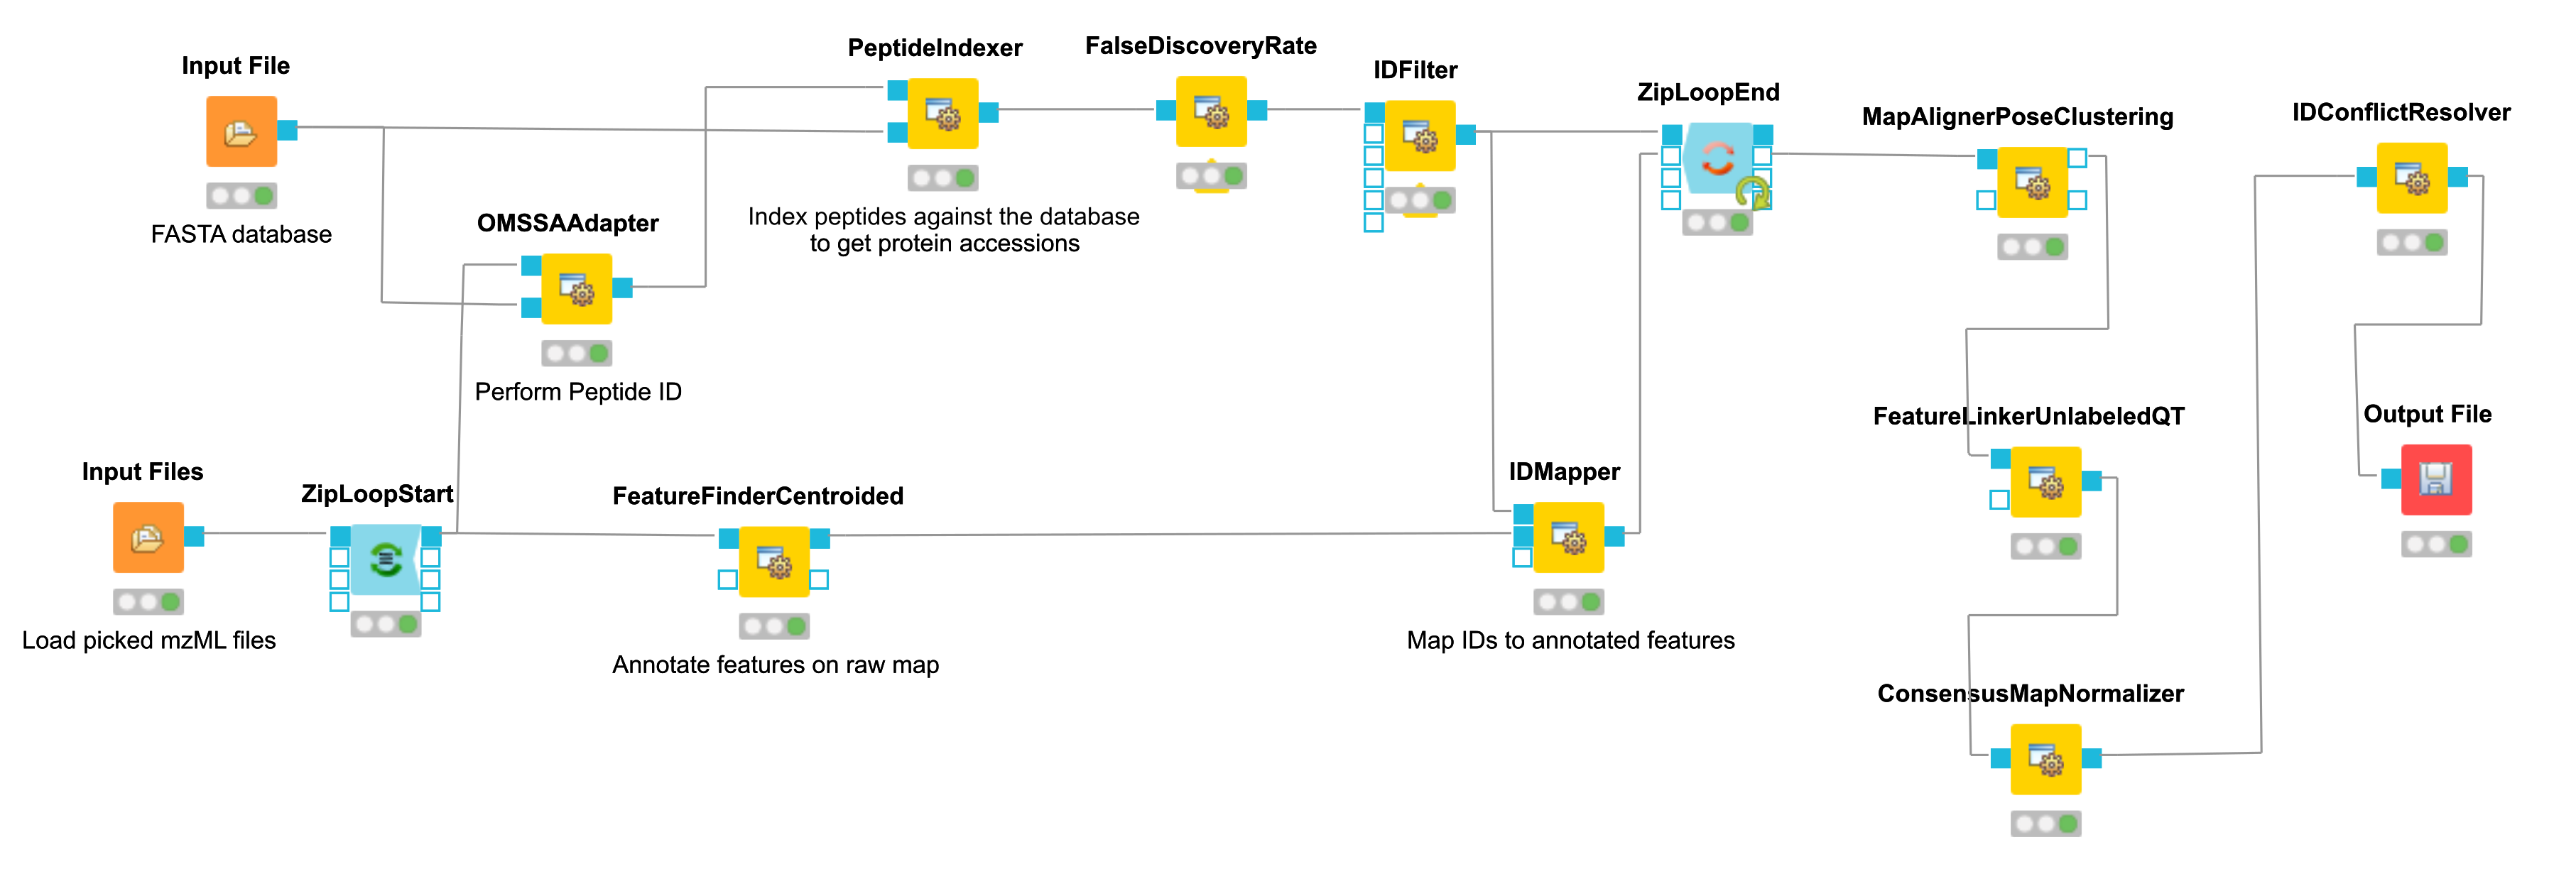
\includegraphics[width=1\textwidth]{graphics/labelfree/iPRG/iPRG_lfq.png}
  \caption{KNIME data analysis of iPRG LFQ data.}
  \label{fig:iPRG_lfq}
\end{figure}

\noindent The iPRG LFQ workflow (Fig. \ref{fig:iPRG_lfq}) consists of an identification and a quantification part. The identification is achieved by searching the computationally calculated MS2 spectra from a sequence database (\KNIMENODE{Input File} node, here with the given database from iPRG, \directory{\IPRGFOLDER / database / iPRG2015\_target\_decoy\_nocontaminants.fasta}) against the MS2 from the original data (\KNIMENODE{Input Files} node with all mzMLs following \directory{\IPRGFOLDER / datasets / JD\_06232014\_sample*.mzML}) using the \KNIMENODE{OMSSAAdapter}.
\note{If you reproduce at home, you have to download the iPRG data in mzML format and perform Peakpicking on it. Or convert and pick the raw data with msconvert.}
Afterwards the results are scored using the \KNIMENODE{FalseDiscoveryRate} and filtered to obtain only unique peptides (\KNIMENODE{IDFilter} TODO why? restriction of MSstats?). The quantification is achieved by the \KNIMENODE{FeatureFinderCentroided}, which performs feature finding on the maps. In the end the quantification results are combined with the filtered identification results (\KNIMENODE{IDMapper}). Further a linear retention time alignment is performed (\KNIMENODE{MapAlignerPoseClustering}), followed by the feature linking process (\KNIMENODE{FeatureLinkerUnlabledQT}). The \KNIMENODE{ConsensusMapNormalizer} is used to normalize the intensities via robust regression over a set of samples (maps) and the \KNIMENODE{IDConflictResolver} assures that only one identification (best score) is associated with a feature. The output of this workflow is a consensusXML file, which can now be converted using the \KNIMENODE{MSstatsConverter} (see \ref{sec:MSstatsConversion}). 

\subsubsection{Experimental design}
\noindent As mentioned before, the downstream analysis can be performed using MSstats. In this case an experimental design has to be specified for the OpenMS workflow. The structure of the experimental design used in OpenMS in case of the iPRG dataset is specified in table \ref{t:Experimental_design_iPRG}. Further, an explanation of the variables can be found in table \ref{t:Experimental_design_exp}. 

\begin{table}[!ht]
\centering
\small
\caption{OpenMS Experimental design for the iPRG2015 dataset. Caution, in the original filenames, the first sample had a hyphen "-" as a separator between sample and biological replicate, the rest of the files had an underscore "\_". The common prefix was omitted.}
\label{t:Experimental_design_iPRG}
\begin{tabular}{lllll}
Fraction\_Group & Fraction           & Spectra\_Filepath     & Label & Sample \\
1               & 1                  & Sample1-A             & 1     & 1      \\
2               & 1                  & Sample1-B             & 1     & 2      \\
3               & 1                  & Sample1-C             & 1     & 3      \\
4               & 1                  & Sample2-A             & 1     & 4      \\
5               & 1                  & Sample2-B             & 1     & 5      \\
6               & 1                  & Sample2-C             & 1     & 6      \\
7               & 1                  & Sample3-A             & 1     & 7      \\
8               & 1                  & Sample3-B             & 1     & 8      \\
9               & 1                  & Sample3-C             & 1     & 9      \\
10              & 1                  & Sample4-A             & 1     & 10     \\
11              & 1                  & Sample4-B             & 1     & 11     \\
12              & 1                  & Sample4-C             & 1     & 12     \\
                &                    &                       &       &        \\
                &                    &                       &       &        \\
Sample          & MSstats\_Condition & MSstats\_BioReplicate &       &        \\
1               & 1                  & 1                     &       &        \\
2               & 1                  & 2                     &       &        \\
3               & 1                  & 3                     &       &        \\
4               & 2                  & 4                     &       &        \\
5               & 2                  & 5                     &       &        \\
6               & 2                  & 6                     &       &        \\
7               & 3                  & 7                     &       &        \\
8               & 3                  & 8                     &       &        \\
9               & 3                  & 9                     &       &        \\
10              & 4                  & 10                    &       &        \\
11              & 4                  & 11                    &       &        \\
12              & 4                  & 12                    &       &       
\end{tabular}
\end{table}

\begin{table}[!ht]
\centering
\small
\caption{Experimental design explanation}
\label{t:Experimental_design_exp}
\begin{tabularx}{\textwidth}{l|X}
\textbf{variables} & \textbf{value} \\ 
\hline \\
\textit{Fraction\_Group} &  Index used to group fractions and source files.  \\
\textit{Fraction} & 1st, 2nd, .., fraction. Note: All runs must have the same number of fractions. \\
\textit{Spectra\_Filepath} & Path to mzML files \\
\textit{Label} & label-free: always 1 \\
\textit{} & TMT6Plex: 1...6 \\
\textit{} & SILAC with light and heavy: 1..2 \\
\textit{Sample} & Index of sample measured in the specified label X, in fraction Y of fraction group Z. \\
\textit{Conditions} & Further specification of different conditions (e.g. MSstats\_Condition; MSstats\_BioReplicate) \\
\end{tabularx}
\end{table}

\noindent The conditions are highly dependent on the experiment and which kind of analysis you want to use. For the MSstats analysis it has to be clear which sample belongs to which condition and if there are biological replicates. This can be specified in further condition columns as shown in table \ref{t:Experimental_design_exp}. For a detailed description of the MSstats-specific
terminology, see their documentation e.g. in the R vignette.

\subsubsection{Conversion and downstream analysis}
\label{sec:MSstatsConversion}

Conversion of the OpenMS-internal consensusXML format (which is an aggregation of quantified and possibly identified features across several MS-maps) to a table (in MSstats-conformant CSV format) is very easy. Let's create a new KNIME workflow for that first. Then, just run the \KNIMENODE{MSstatsConverter} node with a consensusXML and the manually created (e.g. in Excel) experimental design as inputs (loaded via \KNIMENODE{Input File} nodes). Data can be found under \directory{\IPRGFOLDER / MSstats}, first input is \textit{iPRG\_lfq.consensusXML} which was generated for you by a long run of the \textit{iPRG\_lfq.knwf} workflow (seen in Fig.~\ref{fig:iPRG_lfq}), second input is the \textit{iPRG\_experimental\_design\_raw.tsv} TODO why is it called raw? and remember to fix the spelling error in design. Put in the following parameters to match the given experimental design file and to use a simple summing for peptides that elude in multiple features (with the same charge state, i.e. m/z value).
\begin{center}
	\begin{tabular}{l|l}
		\textbf{parameter} & \textbf{value} \\ \hline
		\textit{msstats\_bioreplicate} & MSstats\_Bioreplicate \\
		\textit{msstats\_condition} & MSstats\_Condition \\
		\textit{labeled\_reference\_peptides} & false \\
		\hl{\textit{retention\_time\_summarization\_method}} & sum\\
	\end{tabular}
\end{center}

The downstream analysis of the peptide ions with MSstats is performed in several
steps. These steps are reflected several KNIME R nodes, which consume
the output of \KNIMENODE{MSstatsConverter}. The outline of the workflow can be
seen in Figure~\ref{fig:msstats_workflow}.

\begin{figure}[htbp]
	\centering
	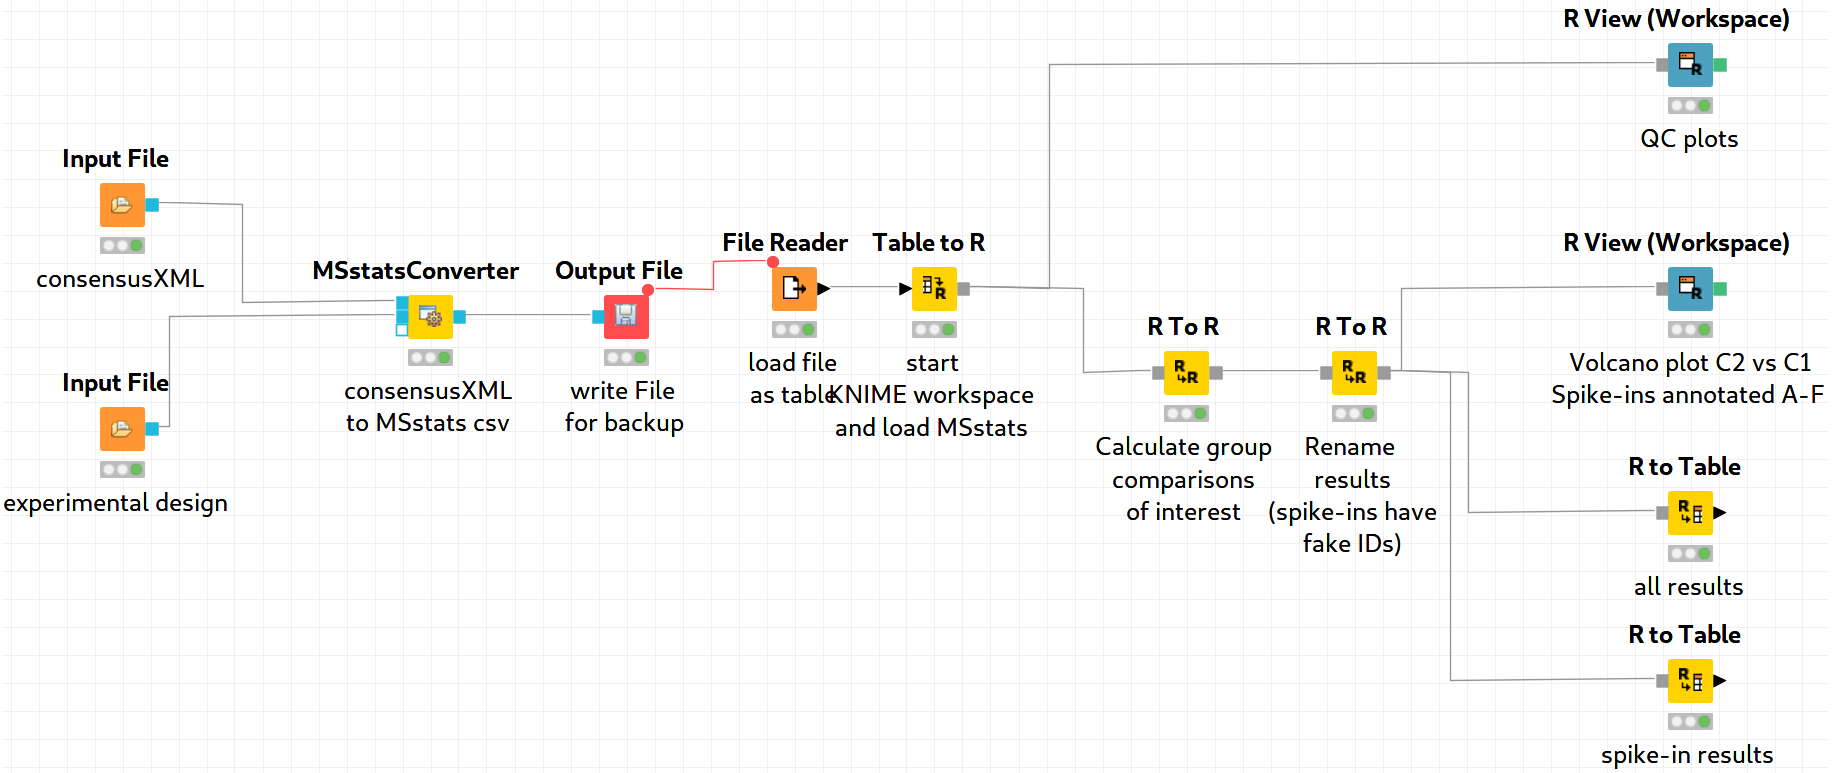
\includegraphics[width=0.9\textwidth]{graphics/labelfree/msstats/MSstats.png}
	\label{fig:msstats_workflow}
	\caption{MSstats analysis using KNIME. The individual steps (Preprocessing,
	Group Comparisons, Result Data Wrangling, and Export) are split
among several consecutive nodes.}
\end{figure}


\paragraph{Preprocessing}
The first node performs preprocessing on the input data. The command
\begin{lstlisting}
quant <- OpenMStoMSstatsFormat(data, removeProtein_with1Feature = FALSE)
\end{lstlisting}
allows further preparation of the data produced by \KNIMENODE{MSstatsConverter} before the actual analysis is performed. In this example, the 
lines with proteins, which were identified with only one feature, were retained. They could be removed as an alternative.

Most importantly, the following line:
\begin{lstlisting}
processed.quant <- dataProcess(quant, censoredInt = 'NA')
\end{lstlisting}
transforms the data into a format that is understood by MSstats.
\texttt{dataProcess} is one of the most important functions that the
R package provides. The function performs the following steps:
\begin{enumerate}
	\item
	Logarithm transformation of the intensities
	\item
	Normalization
	\item
	Feature selection
	\item
	Missing value imputation
	\item
	Run-level summarization
\end{enumerate}
In this example here, we just state that missing intensity values are represented by the NA string. 


\paragraph{Group Comparison}
The goal of the analysis is the determination of differentially-expressed
proteins among the different conditions C1-C4.
We can specify the comparisons that we want to make in a
\emph{comparison matrix}. For this, let's consider the following example:
\begin{equation}
	\begin{pmatrix}
	-1 & 1  & 0 & 0 \\
	-1 & 0  & 1 & 0 \\
	-1 & 0  & 0 & 1 \\
	 0 & -1 & 0 & 1 \\
	 0 & 0  & -1 & 1 \\
	\end{pmatrix}
\end{equation}
This matrix has the following properties:
\begin{itemize}
	\item
	The number of rows equals the number of comparisons that we want to
	perform, the number of columns equals the number of conditions
	(here, column 1 refers to C1, column 2 to C2 and so forth).
	\item 
	The entries of each row consist of exactly one 1 and one -1, the
	rest must be 0.
	\item 
	The condition with the entry 1 constitutes the enumerator
	of the log2 fold-change. The one with entry -1 denotes the 
	denominator.
	Hence, the first row states that we want calculate
	$\log \frac{\text{C}_2}{\text{C}_1}$.
\end{itemize}

We can generate such a matrix in R using the following code snippet:
\begin{lstlisting}
	comparison1<-matrix(c(-1,1,0,0),nrow=1)
	comparison2<-matrix(c(-1,0,1,0),nrow=1)
	comparison3<-matrix(c(-1,0,0,1),nrow=1)
	comparison4<-matrix(c(0,-1,1,0),nrow=1)
	comparison5<-matrix(c(0,-1,0,1),nrow=1)
	comparison6<-matrix(c(0,0,-1,1),nrow=1)
	comparison <- rbind(comparison1, comparison2, comparison3, comparison4, comparison5, comparison6)
	row.names(comparison)<-c("C2-C1","C3-C1","C4-C1","C3-C2","C4-C2","C4-C3")
\end{lstlisting}
Here, we assemble each row in turn, concatenate them at the end, and provide row names for labeling
the rows with the respective condition.

In MSstats, the group comparison is then performed with the following line:
\begin{lstlisting}
	test.MSstats <- groupComparison(contrast.matrix=comparison, data=processed.quant)
\end{lstlisting}
No more parameters need to be set for performing the comparison.

\paragraph{Result Processing}
In the next node, the results are being processed. The following code snippet:
\begin{lstlisting}
	test.MSstats.cr <- test.MSstats$ComparisonResult
	
	# Rename spiked ins to A,B,C....
	pnames <- c("A", "B", "C", "D", "E", "F")
	names(pnames) <- c(
	"sp|P44015|VAC2_YEAST",
	"sp|P55752|ISCB_YEAST",
	"sp|P44374|SFG2_YEAST",
	"sp|P44983|UTR6_YEAST",
	"sp|P44683|PGA4_YEAST",
	"sp|P55249|ZRT4_YEAST"
	)
	
	test.MSstats.cr.spikedins <- bind_rows(
	test.MSstats.cr[grep("P44015", test.MSstats.cr$Protein),],
	test.MSstats.cr[grep("P55752", test.MSstats.cr$Protein),],
	test.MSstats.cr[grep("P44374", test.MSstats.cr$Protein),],
	test.MSstats.cr[grep("P44683", test.MSstats.cr$Protein),],
	test.MSstats.cr[grep("P44983", test.MSstats.cr$Protein),],
	test.MSstats.cr[grep("P55249", test.MSstats.cr$Protein),]
	)
	# Rename Proteins
	test.MSstats.cr.spikedins$Protein <- sapply(test.MSstats.cr.spikedins$Protein, function(x) {pnames[as.character(x)]})
	test.MSstats.cr$Protein <- sapply(test.MSstats.cr$Protein, function(x) {
	
	x <- as.character(x)
	
	if (x %in% names(pnames)) {
	
	return(pnames[as.character(x)]) 
	} else {
	return("")
	}
	})
\end{lstlisting}
will rename the spiked-in proteins to A,B,C,D,E, and F and remove the name of other proteins, which will be beneficial for the subsequent visualization.


\paragraph{Export}
The last two snippets will export the results to a textual representation and volcano plots for further inspection.

\subsubsection{Result}
An excerpt of the main result of the group comparison can be seen in Figure~\ref{fig:msstats_1}.

\begin{figure}[htbp]
	\centering
	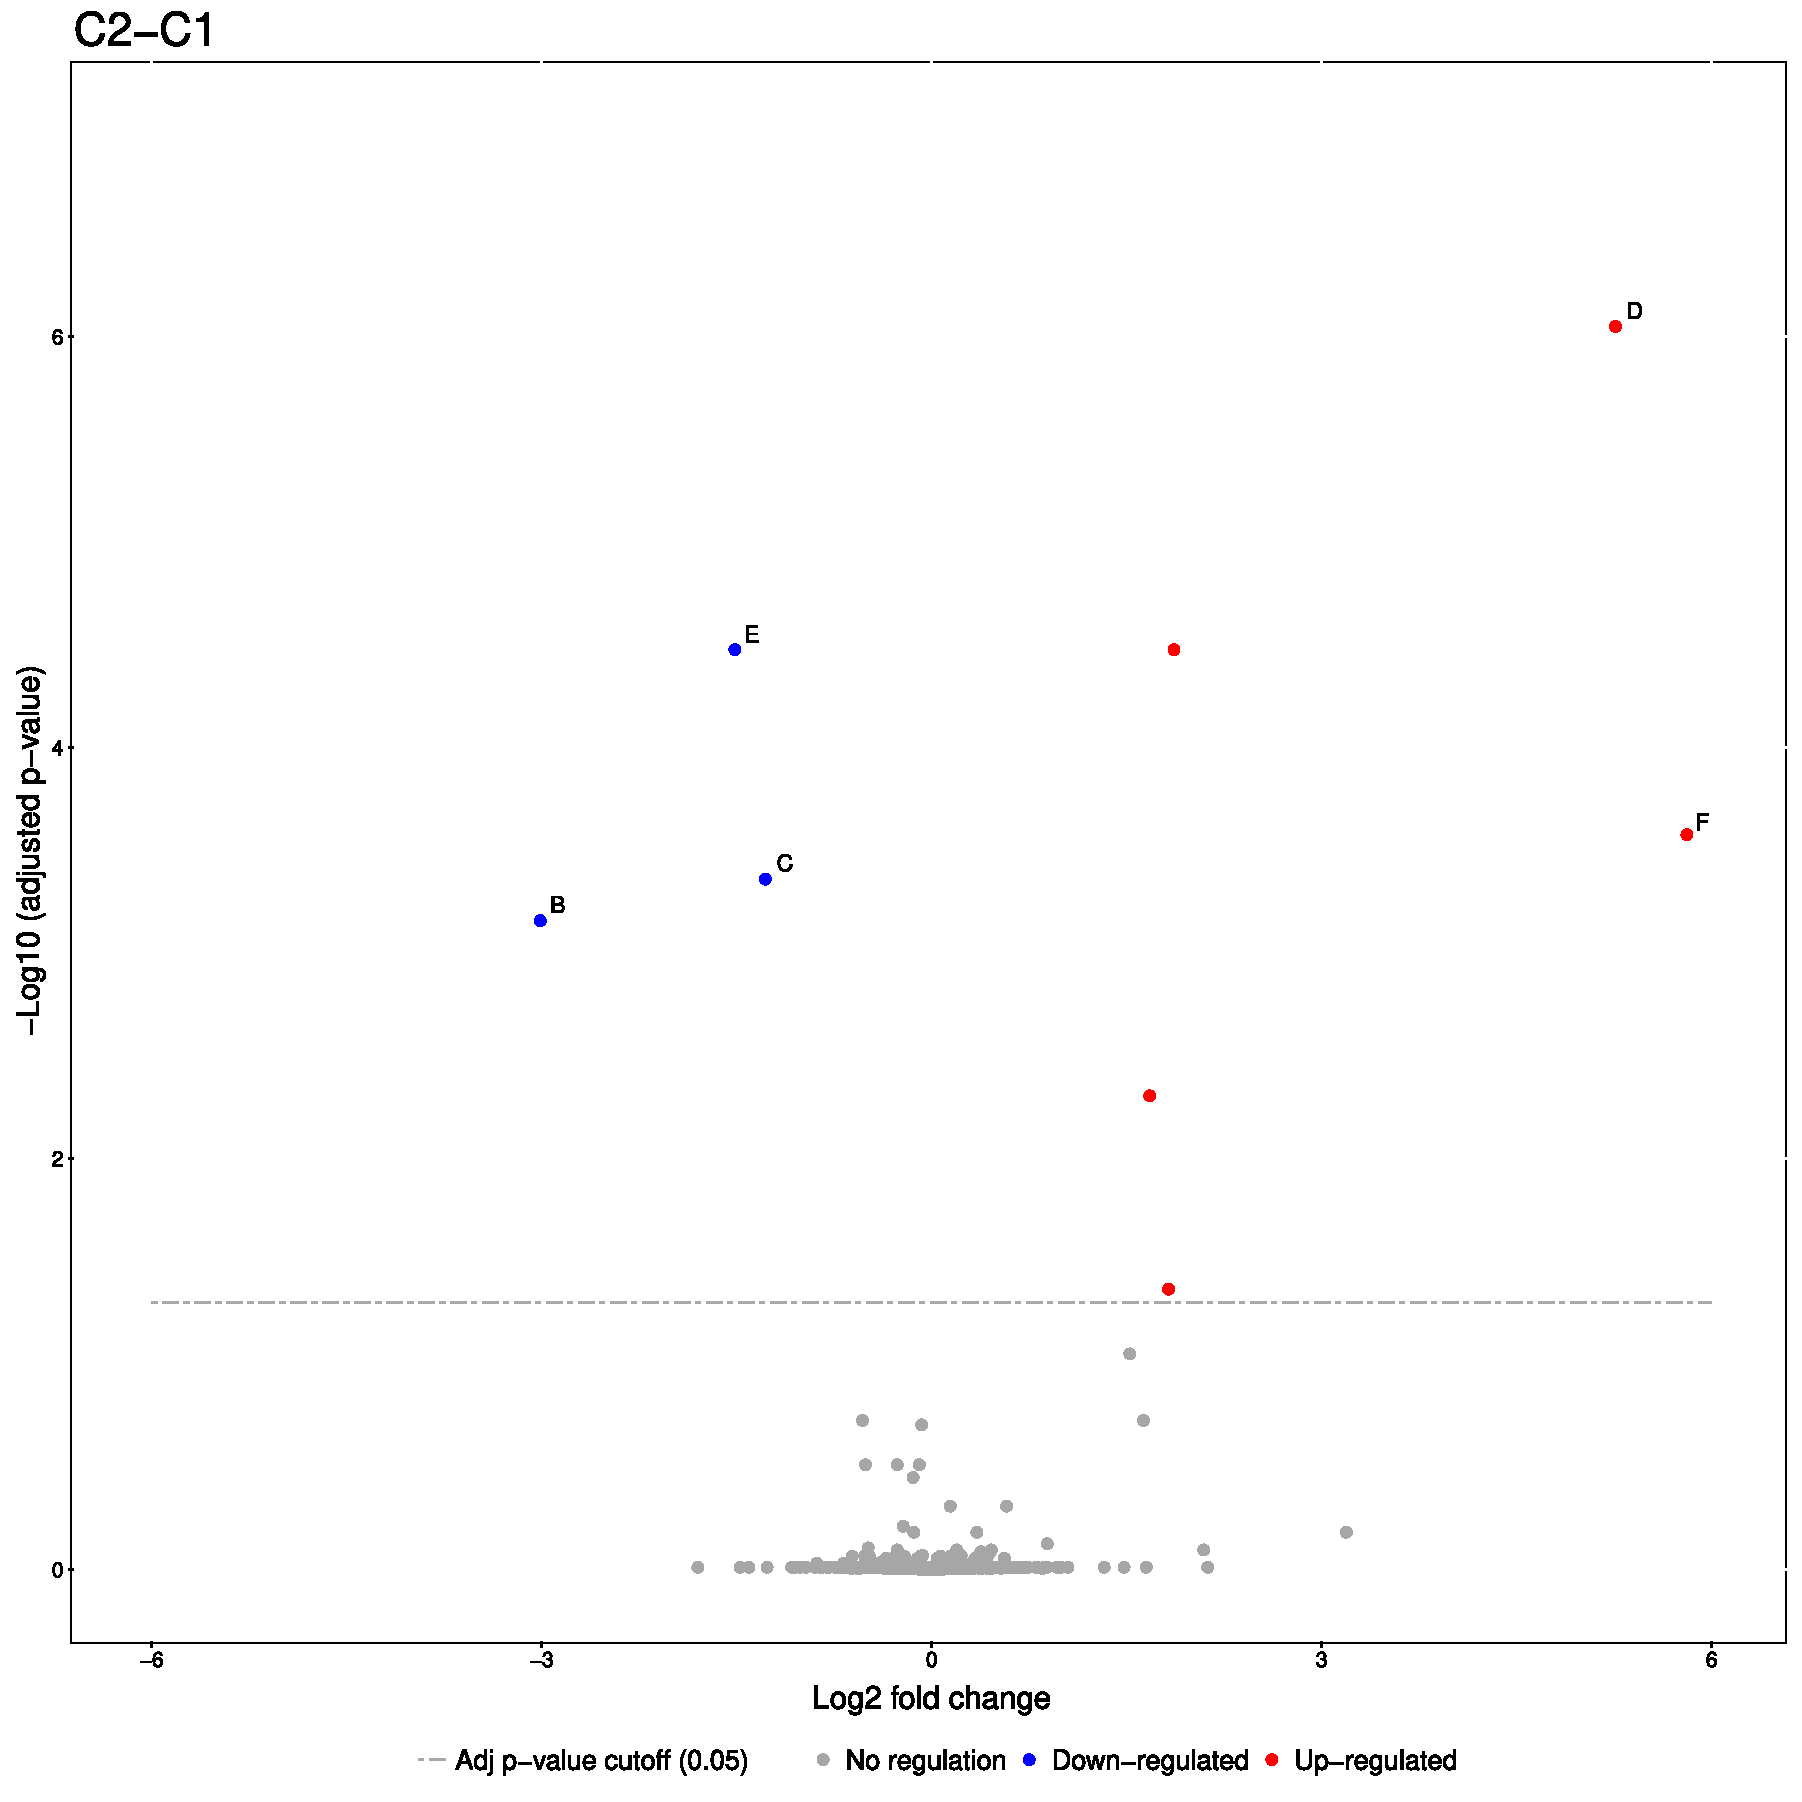
\includegraphics[width=0.45\textwidth]{graphics/labelfree/msstats/c2_c1.pdf}
	\qquad
	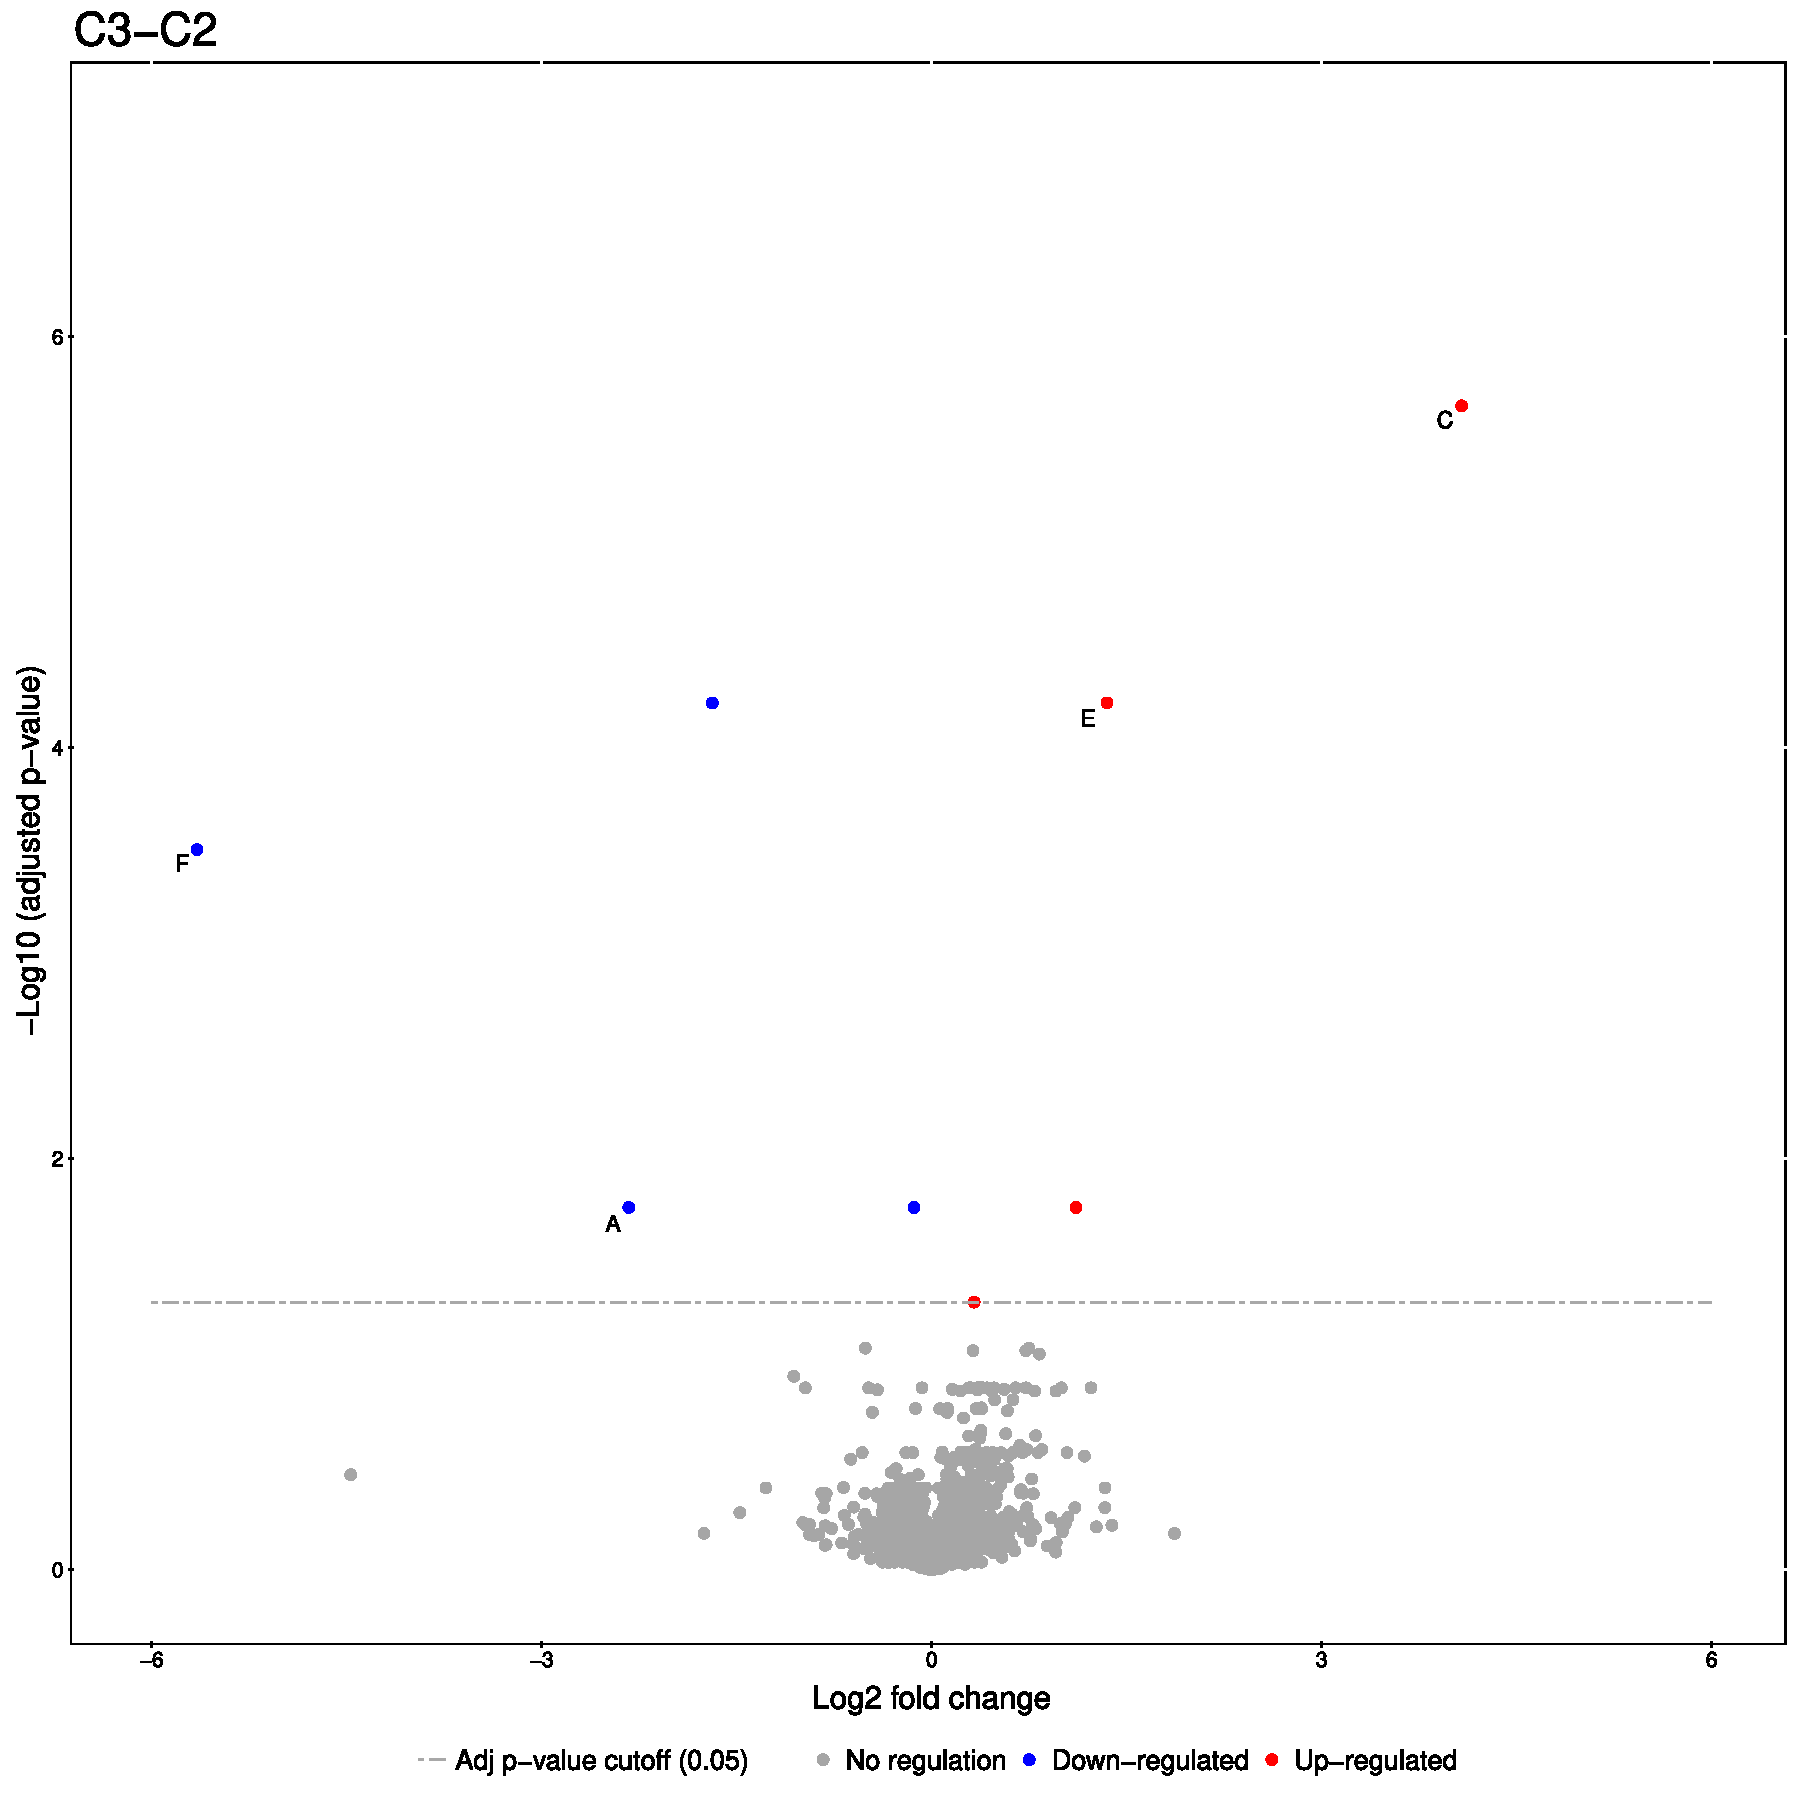
\includegraphics[width=0.45\textwidth]{graphics/labelfree/msstats/c3_c2.pdf}
	\caption{Volcano plots produced by the Group Comparison in MSstats}
	\label{fig:msstats_1}
\end{figure}

The Volcano plots show differently expressed spiked-in proteins. In the left plot, which shows
the fold-change C2-C1, we
can see the proteins D and F (\texttt{sp|P44983|UTR6\_YEAST}
and \texttt{sp|P55249|ZRT4\_YEAST}) are significantly over-expressed in C2, while
 the proteins B,C, and E (\texttt{sp|P55752|ISCB\_YEAST}, \texttt{sp|P55752|ISCB\_YEAST},
 and \texttt{sp|P44683|PGA4\_YEAST}) are under-expressed.
 In the right plot, which shows the fold-change ratio of C3 vs. C2, we
 can see the proteins E and C (\texttt{sp|P44683|PGA4\_YEAST} and \texttt{sp|P44374|SFG2\_YEAST})
 over-expressed and the proteins A and F (\texttt{sp|P44015|VAC2\_YEAST} and
 \texttt{sp|P55249|ZRT4\_YEAST}) under-expressed.


%"sp|P44015|VAC2_YEAST",
%"sp|P55752|ISCB_YEAST",
%"sp|P44374|SFG2_YEAST",
%"sp|P44983|UTR6_YEAST",
%"sp|P44683|PGA4_YEAST",
%"sp|P55249|ZRT4_YEAST"





